%!TEX root = main.tex

\section*{Introduction}

Genetic clustering algorithms are a commonly used approach to describe genetic structure among populations, reflecting the cumulative effects of isolation, connectivity (i.e., genetic migration), selection, and genetic drift.  The capacity of such algorithms to differentiate populations is limited by the extent of genetic differentiation among populations and the capacity to resolve those differences given the available marker set and sample sizes from the respective populations.  Based on an initial description of genetic structure, ecologists are frequently interested in describing patterns of genetic movement among populations, often inferred from the mismatch between the sampling location and genetic origins of a given animal \citep{paetkau1995microsatellite,wilson2003bayesian}.  Describing such patterns of movement have many implications, influencing evolutionary processes, disease dynamics \citep{huestis2019windborne}, or patterns of invasive species expansion.

	In using clustering algorithms to describe genetic structure among natural populations, researchers frequently identify individuals with complex ancestry patterns (i.e., the proportion of an individual’s genome assigned to sampled populations, sensu \citealt{pritchard2000inference}) that demonstrate mixed associations to multiple populations.  Various processes could contribute to such mixed associations.  Most simplistically, individuals may represent the influences of gene flow among populations, occurring in recent or prior generations, with the observed complex ancestry patterns accurately representing contributions from multiple populations included in the study.  However, alternative processes could also create similarly complex ancestry patterns.  For example, individuals may have genomic associations to unsampled populations as immigrants or as descendant of immigrant from unsampled populations \citep{pritchard2000inference,beerli2004effect}.  Yet a limitation of clustering algorithms is that exogenous immigrants can only be associated to populations represented within the sample.  Similarly, individuals with mixed associations may reflect a discrepancy between the genetic structure as described by the analysis and the underlying ecological process creating patterns of genetic differentiation (e.g., when clinal systems governed by isolation by distance are described as discrete genetic clusters).  Finally, such patterns may represent a limitation of the statistical power of the genetic data, as a function of both the marker set and sample size, to resolve the true underlying patterns of genetic structure.  The challenge for researchers then becomes correctly identifying the ecological process by which similar, complex ancestry patterns were created.  
	
Pairing empirical data with closely derived simulation-based approaches has been long recognized as a tool to help guide the interpretation of empirical data and define the limitations of the available data \citep{vaha2006efficiency,anderson2008improved,latch2011fine}.  Mirroring empirical datasets with forward-in-time simulations often implement sampling with replacement (e.g. citations).  However, sampling with replacement implicitly increases the pairwise genetic distance (i.e., FST) among populations and inflates the perceived ability to correctly assign individuals back to source populations \cite{almudevar2000exact,anderson2008improved}.  \textcolor{red}{Seems like 2 additional sentences here would be appropriate to draw from a study that has demonstrated this process.}  The effects of overestimating our ability to resolve populations creates individuals that discretely align with simulated populations.  These issues could be addressed with simulations that fix observed genetic differences among populations by sampling from the empirical data without replacement (citations for simulation frameworks that use this approach).
  Beyond simply evaluating the resolution of discrete populations in a simulated framework, researchers may also be interested in how individuals of admixed ancestry are genetically characterized.  Recognizing that connectivity among genetically distinct populations may be relatively rare, researchers can gain additional insights into the frequency of immigration by also identifying descendants of migrants among study populations (directly [F1 hybrids] or advanced hybrids reflecting the effect of backcrossing across multiple generations [BC1, \ldots, BCX]).  The process of recombination during meiosis creates a distribution of expected associations to parental populations among advanced hybrid classes. Treating linked loci as independent can lead to the false interpretation that the association of advanced hybrid classes to parental population occur strictly as discrete distributions.  Therefore, in evaluating descendants of migrants within a simulated framework, it is imperative to take into consideration the pattern of linkage among loci available for analysis.
	In response to these needs, we developed gscramble – an approach to simulate genotypes that minimizes bias associated with forward-in-time simulations by sampling alleles from respective populations without replacement, thus preserving the genetic differences observed in the empirical dataset.  Further, by simulating individual genotypes based on user-defined pedigrees, gscramble allows for the simulation of admixed genotypes of varying degrees of complexity while allowing the tracking of haplotype blocks from source populations within the specified pedigree.  By integrating species-specific recombination rates, gscramble simulates biologically informed genotypes that mirror empirical data.  We develop and illustrate gscramble with use of single nucleotide polymorphic (SNP) genotypes.


Can we say something about Anthony Almudevar's visionary method for GSI power assessment \citep{almudevar2000exact}


\section*{Methods}

Something here.

\subsection*{Genomic Simulation Pedigrees}

For the purposes here, we define blah, blah.

\subsection*{Another subsection}



\subsection*{And a third}

Blah, blah blobbity blah.


\begin{figure*}
\begin{center}
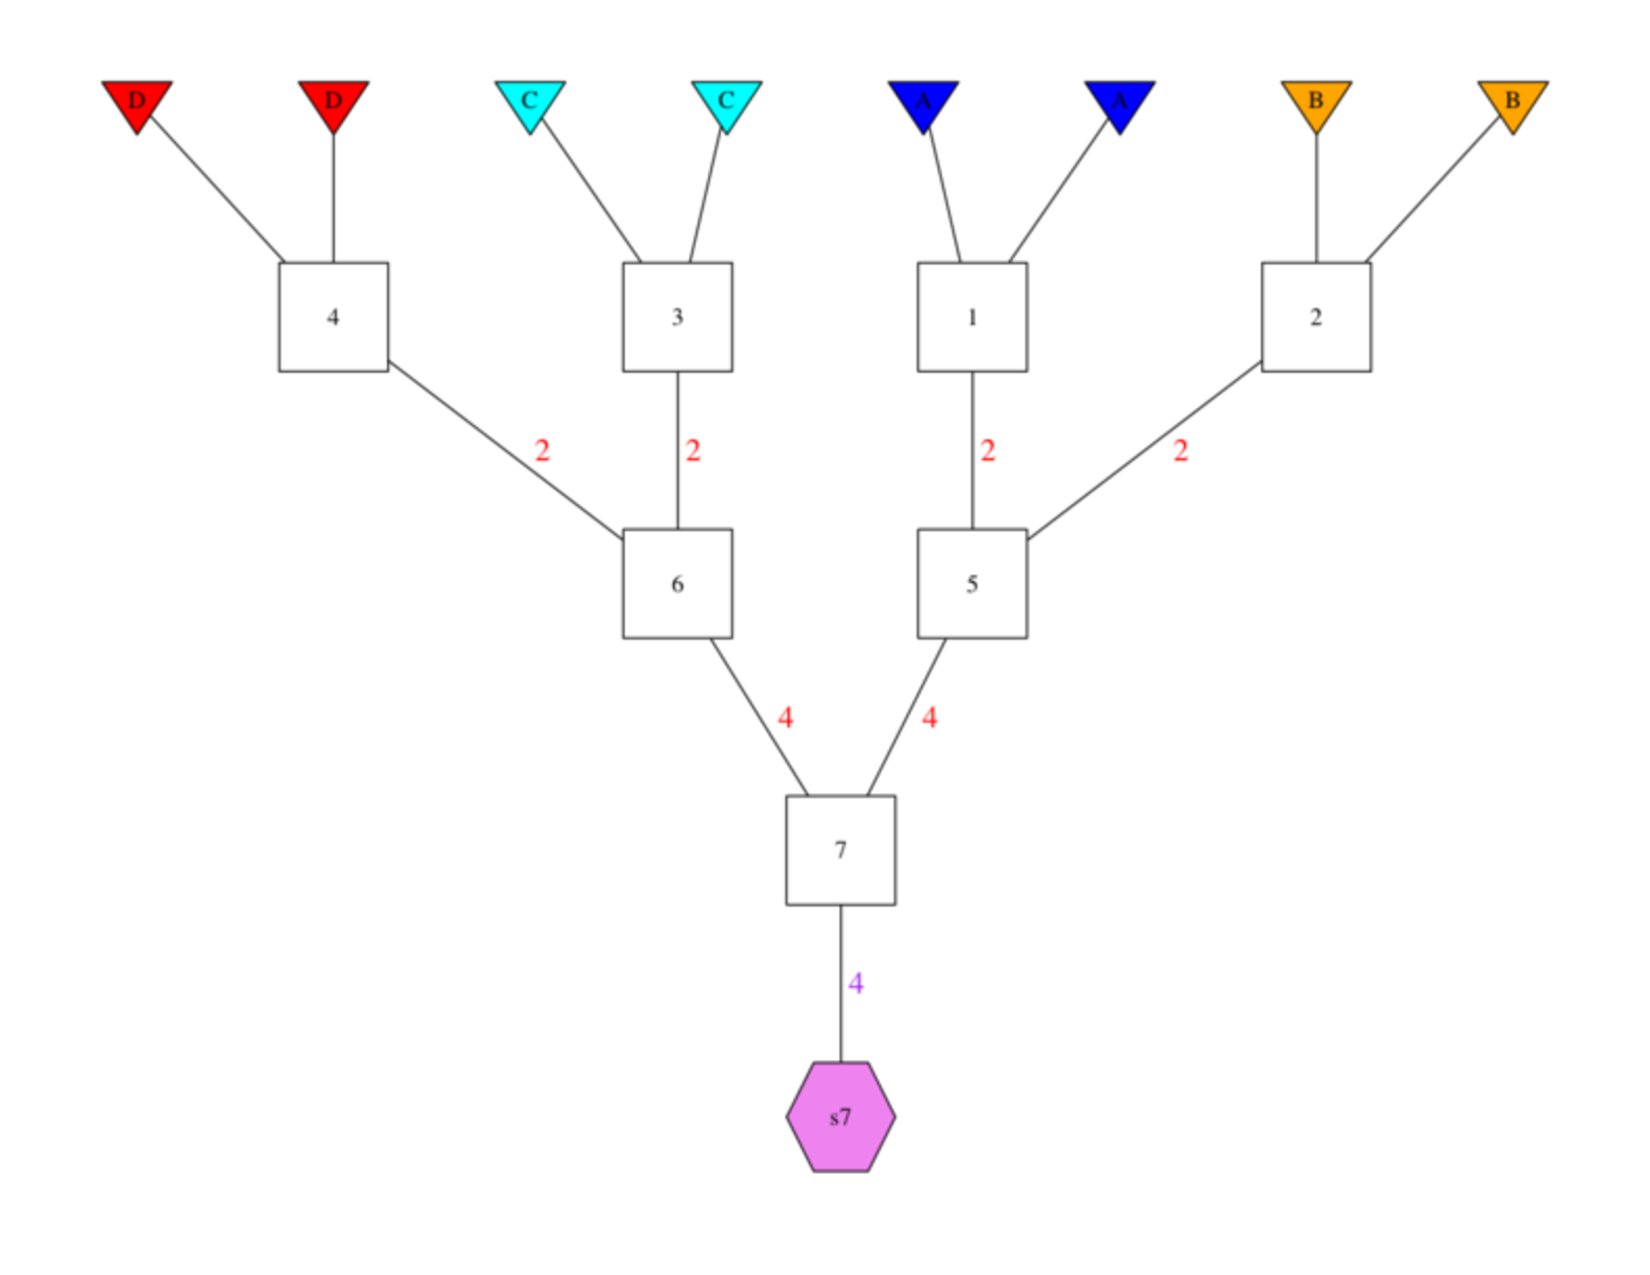
\includegraphics[width=0.8\textwidth]{images/gsp4-700.pdf}
\end{center}
\caption[]{Stick this thing in somewhere}
\end{figure*}




\section*{Discussion}
Hey! Let's discuss this!



\section*{Acknowledgements}
We thank etc. etc.   Contribution number  mHAVEAGAS-003